\subsection{Decision Tree}

We have created decision trees using the four different kinds of input as described in section \ref{classification} on page \pageref{classification}. The decision tree based on using all the attributes can be seen in Figure \ref{decisionTreeX}.%Some of the output of these decision trees can be seen in Figure \ref{decisionTreeX}.

\begin{figure}[H]
\center
	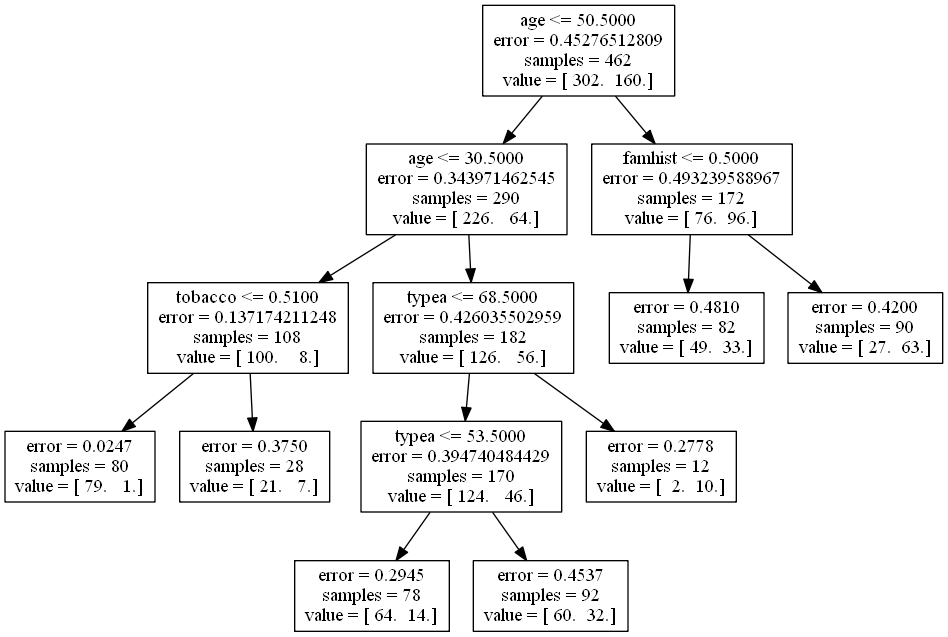
\includegraphics[scale=0.25]{pictures/Decision_Tree_X.png}
	\caption{Decision tree looking at all attributes.}
	\label{decisionTreeX}
\end{figure}

Now one can use such decision trees to classify data objects, which is simply done by following branches of the tree, until one reaches a leaf, which then either represent people with negative or positive CHD.

Therefore one can go through each data object, and compare how it will be classified according to the decision trees and which value it truly has. This way we have calculated the misclassification error, which can be seen in Table \ref{decisionTreeErrorRate}

The table below shows the error rate for the other computed decision trees as well.% Unfortunately they would not fit into a report in a readable manor.
\begin{table}[H]
\begin{longtable}{lc}\hline
Result from: & Mis-classification rate \\ \hline
All attributes & 25,1\% \\ 
Feature selected attributes & 25,1\% \\ 
All principal components & 21,4\% \\ 
Two most important PC & 28,8\% \\ \hline
\end{longtable}
\caption{Mis-classification rates of decision trees.}
\label{decisionTreeErrorRate}
\end{table}

For making these decisions trees, we have used the whole data set as input. Furthermore, we have defined that the a node need to contain at least 100 objects in order to be split up. As we use the whole data set as input for the decision tree, and we also calculate the mis-classification rate according to how well the tree can classify objects from our data set, then by defining a very low lower bound for when to split up nodes, we can get a very high classification rate.
